\documentclass[tikz,border=10pt]{standalone}
\begin{document}
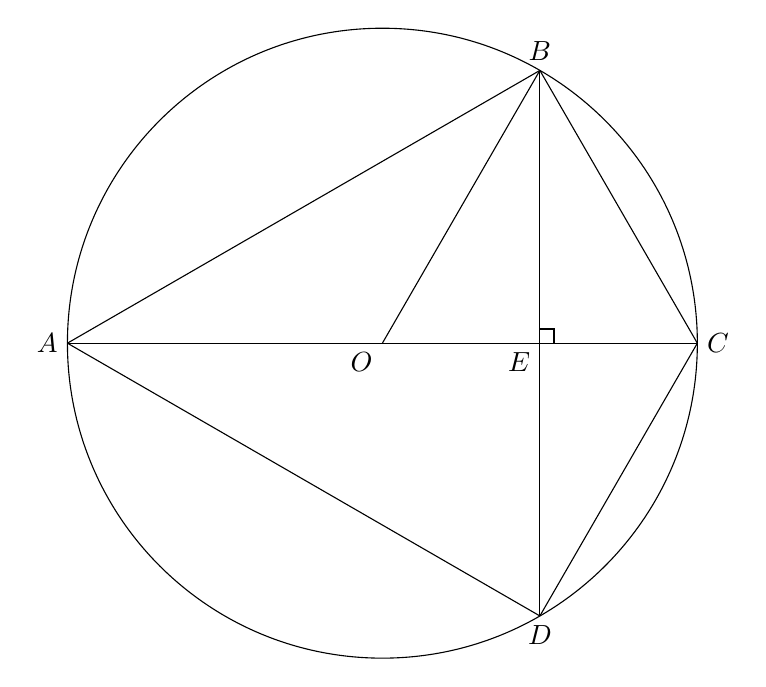
\begin{tikzpicture}[scale=1]

% Points
\coordinate (O) at (0,0);
\coordinate (A) at (-4,0);
\coordinate (C) at (4,0);
\coordinate (B) at (2,3.464);
\coordinate (D) at (2,-3.464);
\coordinate (E) at (2,0);

% Circle
\draw (O) circle (4);

% Segments
\draw (A) -- (C);
\draw (A) -- (B);
\draw (A) -- (D);
\draw (O) -- (B);
\draw (B) -- (E);
\draw (E) -- (D);
\draw (B) -- (C);
\draw (D) -- (C);

% Right-angle mark at E
\draw (2,0) ++(0.18,0) -- ++(0,0.18) -- ++(-0.18,0);

% Labels
\node[left] at (A) {$A$};
\node[right] at (C) {$C$};
\node[above] at (B) {$B$};
\node[below] at (D) {$D$};
\node[below left] at (O) {$O$};
\node[below left] at (E) {$E$};

\end{tikzpicture}
\end{document}
